\section{Auswertung}
\label{sec:Auswertung}

\subsection{Darstellung der Temperaturverläufe}

Es wurden die Temperaturen, Druckwerte und die Kompressorleistung minütlich 
gemessen. Die gemessenen Daten sind in Tabelle \ref{tab:Messdaten} dargestellt. 

\begin{table}
\centering
\caption{Aufgenommene Messdaten}
\label{tab:Messdaten}
\sisetup{table-format=2.1}
\begin{tabular}{c c c c c c}
\toprule
$t \,/\, \si{\second}$ & $T_1 \,/\, \si{\kelvin}$ & 
$T_2 \,/\, \si{\kelvin}$ & $p_a \,/\, \si{\kilo\pascal}$ & 
$p_b \,/\, \si{\kilo\pascal}$& $P \,/\, \si{\watt}$\\
\midrule
   0 & 294.65 & 294.55 & 490 &  510 & 120\\
  60 & 295.55 & 294.45 & 440 &  650 & 125\\
 120 & 297.05 & 293.15 & 460 &  675 & 126\\
 180 & 298.65 & 291.65 & 470 &  700 & 128\\
 240 & 300.25 & 290.25 & 475 &  725 & 128\\
 300 & 301.75 & 289.25 & 460 &  750 & 125\\
 360 & 303.35 & 288.25 & 445 &  775 & 123\\
 420 & 304.85 & 287.35 & 430 &  800 & 122\\
 480 & 306.25 & 286.35 & 420 &  850 & 122\\
 540 & 307.55 & 285.35 & 400 &  875 & 124\\
 600 & 308.85 & 284.45 & 395 &  900 & 125\\
 660 & 310.05 & 283.45 & 380 &  925 & 125\\
 720 & 311.15 & 282.55 & 370 &  950 & 125\\
 780 & 312.25 & 281.65 & 360 & 1000 & 126\\
 840 & 313.25 & 280.85 & 350 & 1000 & 128\\
 900 & 314.25 & 280.05 & 340 & 1050 & 128\\
 960 & 315.25 & 279.25 & 340 & 1075 & 115\\
1020 & 316.05 & 278.55 & 330 & 1100 & 115\\
1080 & 316.95 & 277.75 & 320 & 1125 & 115\\
1140 & 317.75 & 277.05 & 320 & 1150 & 115\\
1200 & 318.45 & 276.45 & 310 & 1175 & 115\\
1260 & 319.25 & 275.75 & 300 & 1200 & 115\\
1320 & 319.95 & 275.15 & 300 & 1200 & 115\\
1380 & 320.65 & 274.55 & 300 & 1225 & 115\\
1440 & 321.25 & 274.05 & 295 & 1250 & 115\\
1500 & 321.95 & 273.45 & 290 & 1275 & 115\\
1560 & 322.55 & 273.35 & 280 & 1300 & 115\\
1620 & 323.15 & 272.45 & 280 & 1300 & 115\\
1680 & 323.75 & 271.95 & 280 & 1325 & 115\\
\bottomrule
\end{tabular}
\end{table}

Zur Bestimmung der Differentialquotienten $\frac{\symup{d}T_1}{\symup{d}t}$ und 
$\frac{\symup{d}T_2}{\symup{d}t}$ werden die Messdaten mit $T(t)=At²+Bt+C$ 
approximiert. Die durch Python und Matplotlib ermittelten Parameter lauten: 

\begin{align*}
A_1 &= \SI{-6.23+-0.18e-6}{\kelvin\per\squared\second}\\
B_1 &= \SI{28+-0.03e-3}{\kelvin\per\second}\\
C_1 &= \SI{294.113+-0.1113}{\kelvin}
\end{align*}

\begin{align*}
A_2 &= \SI{3.90+-0.17e-6}{\kelvin\per\squared\second}\\
B_2 &= \SI{-20+-0.03e-3}{\kelvin\per\second}\\
C_2 &= \SI{295.132+-0.1077}{\kelvin}
\end{align*}

\begin{figure}
  \centering
  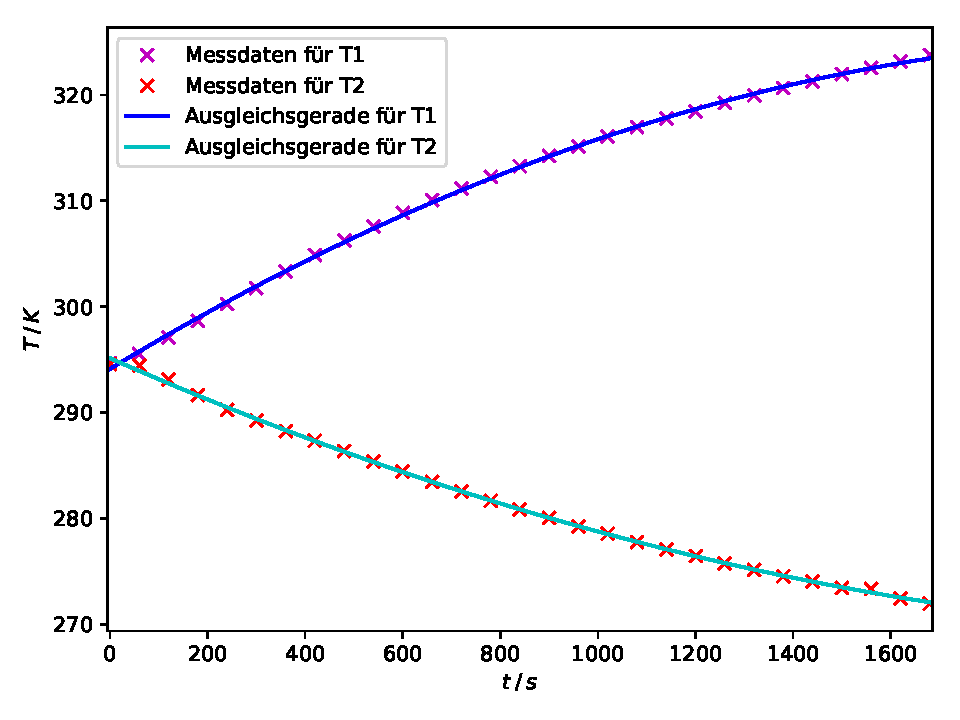
\includegraphics[scale=0.8]{content/plot1.pdf}
  \caption{Temperaturverläufe}
  \label{fig:plot}
\end{figure}

Anhand von Abbildung \ref{fig:plot} ist zu erkennen, dass die Messwerte 
gut zu der geplotteten Funktion passen.

Die Differentialquotienten ergeben sich durch die Ableitung der Fitfunktion: 

\begin{equation*}
\frac{\symup{d}T}{\symup{d}t} = 2A \cdot t + B
\end{equation*}

Die berechneten Werte für die Differentialquotienten für vier Temperaturen
sind in Tabelle \ref{tab:Diff} aufgelistet.

\begin{table}
\centering
\caption{Differentialquotienten}
\label{tab:Diff}
\sisetup{table-format=2.1}
\begin{tabular}{c c c}
\toprule
$t \,/\, \si{\second}$ & $\frac{\symup{d}T_1}{\symup{d}t} \,/\, \SI{e-3}{\kelvin\per\second}$ & 
$\frac{\symup{d}T_2}{\symup{d}t} \,/\, \SI{e-3}{\kelvin\per\second}$\\
\midrule
 120 & 26.50 \pm \,0.30 & -19.06 \pm \,0.30\\
 360 & 23.51 \pm \,0.33 & -17.19 \pm \,0.32\\
 480 & 22.02 \pm \,0.35 & -16.26 \pm \,0.34\\
 600 & 20.52 \pm \,0.37 & -15.32 \pm \,0.36\\
\bottomrule
\end{tabular}
\end{table}

Dabei werden hierbei die Fehler aus den statistischen Fehlern der Fitwerte 
nach 

\begin{equation*}
\symup{\Delta} \frac{\symup{d}T}{\symup{d}t} = \sqrt{(2t\cdot\symup{\Delta} A)² + (\symup{\Delta} B)²}
\end{equation*}

berechnet.

\subsection{Bestimmung der Güteziffern}

Damit die Güteziffer berechnet werden kann, muss zunächst die Wärmekapzitiät
der beiden Wasserreservoire ermittelt werden. Beide Reservoire haben die gleiche 
Wärmekapzitiät, da sie den gleichen Aufbau haben und jeweils mit 
$V = \SI{3+-0.0012}{\liter}$ befüllt sind. Es ergibt sich für die 
Wärmekapzitiät: 

\begin{equation*}
C = C_\text{p} \cdot \rho \cdot V + m_\text{k} \cdot c_\text{k} = 
\SI{13293+-5}{\joule\per\kelvin}
\end{equation*}

Dabei ist $C_p = \SI{4.181}{\joule\per\gram\per\kelvin}$ [4], 
$\rho = \SI{1000}{\gram\per\liter}$ wird angenommen und die Wärmekapazität 
des Reservoires ist gegeben als $c_\text{k} m_\text{k}$ = \SI{750}{\joule\per\kelvin}.
Mit \eqref{eqn:Güteziffer} wird nun die Güteziffern für die 
vier ermittelten Differentialquotienten bestimmt. Die Ergebnisse sind in 
Tabelle \ref{tab:Güte} aufgeführt. 

\begin{table}
\centering
\caption{Güteziffern}
\label{tab:Güte}
\sisetup{table-format=2.1}
\begin{tabular}{c c c c c}
\toprule
$t \,/\, \si{\second}$ & $\frac{\symup{d}T_1}{\symup{d}t} \,/\, \SI{e-3}{\kelvin\per\second}$ & 
$\nu _\text{id}$ & $\nu _\text{re}$ & Abweichung \%\\
\midrule
 120 & 26.50 \pm \,0.30 & 76.17 & 2.80 \pm \,0.03 & 96.32\\
 360 & 23.51 \pm \,0.33 & 20.09 & 2.54 \pm \,0.04 & 87.36\\
 480 & 22.02 \pm \,0.35 & 15.39 & 2.40 \pm \,0.04 & 84.41\\
 600 & 20.52 \pm \,0.37 & 12.66 & 2.18 \pm \,0.04 & 82.78\\
\bottomrule
\end{tabular}
\end{table}

Dabei berechnet sich die ideale Güteziffer nach \eqref{eqn:ideal}. Der 
Fehler der realen Güteziffer ergibt sich nach der Gaußschen 
Fehlerfortpflanzung zu 

\begin{equation*}
\symup{\Delta} \nu = \sqrt{\left(C\cdot \symup{\Delta} \frac{\symup{d}T_1}{\symup{d}t}\right)²+\left(\frac{\symup{d}T_1}{\symup{d}t}\cdot \symup{\Delta} C\right)²}.
\end{equation*}

\subsection{Bestimmung des Massendurchsatzes}

Zur Bestimmung des Massendurchsatzes wird die Verdampfungswärme $L$ benötigt. 
Diese lässt sich durch ein Dampfdruck-Kurve gewinnen. Zu diesem Zweck wird 
$ln({P})$ gegen $\frac{1}{T}$ aufgetragen und eine lineare Ausgleichsgerade
geplottet.
Grafisch aufgetragen ergibt sich die Abbildung \ref{fig:plot2}. 

\begin{figure}
  \centering
  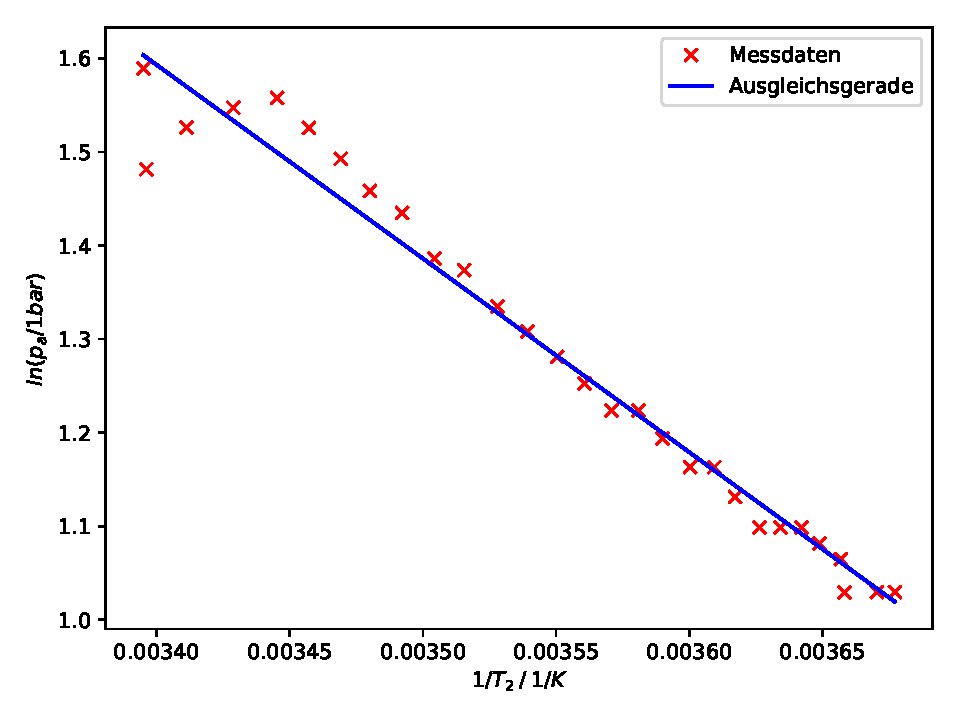
\includegraphics[scale=0.8]{content/plot2.pdf}
  \caption{Dampfdruck-Kurve}
  \label{fig:plot2}
\end{figure}

Die Regressionsparameter ergeben sich an der Form $\ln({p}) = \frac{a}{T} +b$ 
zu:

\begin{align*}
a &= \SI{-2071.13+-73.68}{\kelvin}\\
b &= (\SI{8.64+-0.26}{})
\end{align*}

Nach \eqref{eqn:Verdampfung2} ergibt sich $L_\text{reg} = -a \cdot R$, wobei 
$R$ die allgemeine Gaskonstante ist. Mit 
$R = \SI{8.3144621}{\joule\per\mol\per\kelvin}$ [2], 
ergibt sich:

\begin{equation*}
L_\text{reg} = \SI{17200+-600}{\joule\per\mol}
\end{equation*}

Die Umrechnung dieser Größe mit Bezug auf eine Masse anstatt auf eine
Teilchenzahl, erfolgt mit der molaren Masse $M = \SI{120.913}{\gram\per\mol}$ [3]
und man erhält:

\begin{equation*}
L = \SI{142+-5}{\joule\per\gram}
\end{equation*}

Nach Formel \eqref{eqn:Massendurchsatz} folgen die Massendurchsätze in 
Tabelle \ref{tab:Massendurchsatz}. 

\begin{table}
\centering
\caption{Massendurchsätze}
\label{tab:Massendurchsatz}
\sisetup{table-format=2.1}
\begin{tabular}{c c c}
\toprule
$t \,/\, \si{\second}$ & $\frac{\symup{d}T_2}{\symup{d}t} \,/\, \SI{e-3}{\kelvin\per\second}$ & 
$ \frac{\symup{d}m}{\symup{d}t} \,/\, \si{\gram\per\second}$\\
\midrule
 120 & -19.06 \pm \,0.30 & -1.78 \pm \,0.07\\
 360 & -17.19 \pm \,0.32 & -1.61 \pm \,0.06\\
 480 & -16.26 \pm \,0.34 & -1.55 \pm \,0.06\\
 600 & -15.32 \pm \,0.36 & -1.43 \pm \,0.06\\
\bottomrule
\end{tabular}
\end{table}

Der Fehler des Massendurchsatzes ergibt sich dabei mit der Gaußschen 
Fehlerfortpflanzung zu: 

\begin{equation*}
\symup{\Delta} \frac{\symup{d}m}{\symup{d}t} = 
\sqrt{\left(C\cdot\frac{1}{L}\cdot\symup{\Delta}\frac{\symup{d}T_2}{\symup{d}t}\right)²-
\left(C\cdot\frac{\symup{d}T_2}{\symup{d}t}\cdot\frac{1}{L²}\cdot\symup{\Delta}L\right)²+
\left(\frac{\symup{d}T_2}{\symup{d}t}\cdot \frac{1}{L}\cdot \symup{\Delta} C\right)²} 
\end{equation*}

\subsection{Bestimmung der Kompressorleistung}

Es wird die Kompressorleistung $N$ nach Formel \eqref{eqn:Kompressor} 
bestimmt. Dazu muss $\rho$ aus der idealen Gasgleichung bestimmt werden. 
Durch Umformen folgt: 

\begin{equation*}
\rho = \frac{P_\text{a} \cdot \rho_\text{o} \cdot T_\text{o}}{P_\text{o} \cdot T_2}.
\end{equation*}

Mit $\rho_\text{o} = \SI{5.52}{\gram\per\liter}$ bei $T_\text{o} = \SI{273.15}{\kelvin}$
und $p = \SI{1}{\bar}$ und $\kappa = 1.14$ ergeben sich die Werte, die in
Tabelle \ref{tab:Kompressor} aufgeführt sind.

\begin{table}
\centering
\caption{Kompressorleistung}
\label{tab:Kompressor}
\sisetup{table-format=2.1}
\begin{tabular}{c c c}
\toprule
$t \,/\, \si{\second}$ & $\rho \,/\, \si{\kilo\gram\per\meter³}$ & 
$ N_\text{mech} \,/\, \si{\watt}$\\
\midrule
 120 & 23.63 & 11.9 \pm \,0.5\\
 360 & 23.25 & 15.5 \pm \,0.6\\
 480 & 22.09 & 19.0 \pm \,0.7\\
 600 & 20.92 & 20.5 \pm \,0.9\\
\bottomrule
\end{tabular}
\end{table}